\chapter{Powerups}

The 6 powerups and their implementation will be discussed separately. Most powerups' duration was handled by having 2 variables: The duration of the powerup and the time when the powerup was collected. Then the program would know that a powerup is active or not if:
\[ Now < Duration + StartTime \]
As such, the StartTime would need to be initialised to \textit{Now - Duration}, otherwise all powerups would be active at the start of the game. When a powerup is collected, the StartTime for that powerup would be set to \textit{Now}. Other powerups which do not work with time (such as the bullets, where the player has a limited amount of them) are explicitly stated how they work in their respective section.

The powerup objects were implemented by having an object pool of 10 powerups and these would be spawned at position \textit{[100, 100]} with 0 velocity. Then when a brick is hit, the powerup has a 50\% of appearing and the powerup physics object would be placed upon the brick with velocity \textit{[0, SomeDownwardsVelocity]}. The actual rendered object is placed on the physics object automatically(since this is done each frame). When the powerup ball hits the platform, a random powerup is given to the player with equal probability. The powerup would then be put away from the screen and its velocity reset.

\begin{figure}[H]
	\centering
	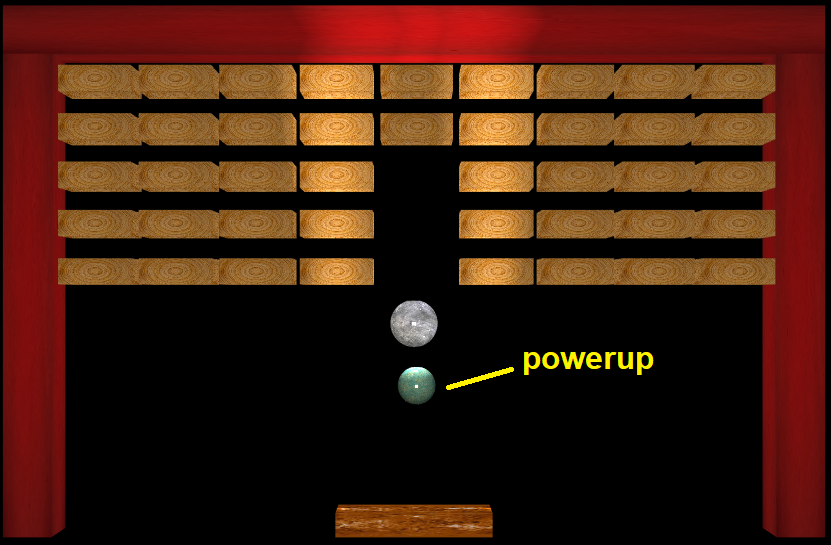
\includegraphics[width=0.7\textwidth]{Images/powerup.png}
	\caption{Image showing the powerup. Notice the light on top caused by the ball's point light}
\end{figure}

\section{Moving trough bricks}
For this powerup, it was a matter of simply making a condition where if the powerup is active (using the time method stated above) the ball's velocity would remain constant when hitting a brick. Then it would be rebounded once it hits the wall or platform. Note: this powerup only works on the main ball, not the additional balls as well. This powerup may be seen in the video at 00:24.

\section{Resizing the platform}
For this, the platform width is changed. This is done by having an \textit{initialWidth} variable as well as a \textit{multiplier} variable which was set to 1.3 (ie the platform will be 1.3x of it's initial size). Then at each frame, the width is changed according to whether the powerup is active or not, and everything regarding the platform depends on this width so it all changes accordingly (such as the point lights' positions).  This powerup may be seen in the video at 00:23.

\section{Additional Balls}
A pool of additional balls was created and, just like the powerups themselves, these were placed away from the screen and set with velocity 0. When the additional ball powerup is collected, this spawns a new ball next to the main ball with the same velocity. The position of the new ball is determined based on the position of the ball with regards to screen space. If the ball is on the left side of the screen, then the additional ball is spawned on the ball's right and vice versa. Important to note is that any powerup which the main balls have, these are not shared by the additional balls. This was to make the additional balls act like basic balls, while the main ball is special. The main ball and additional balls can collide with each other, and when they do, they get reflected so that they go in opposite directions of each other. A check is made in the animate loop so that if the ball starts moving just horizontally (ie gets stuck bouncing between the horizontal walls) it gets a bit of a velocity downwards. This powerup may be seen in the video at 00:30.

\begin{figure}[H]
	\centering
	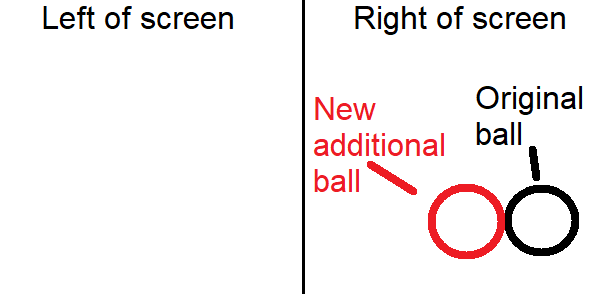
\includegraphics[width=0.7\textwidth]{Images/AdditionalBall.png}
	\caption{Image showing how additional balls are spawned. Since the ball is on the right side of the screen, the new additional ball is spawned on the left of the main ball}
\end{figure}

\section{Slow Ball}
When moving the ball in the animate loop, a check is made to see if the slow moving powerup is active. If it is, the ball moves at half speed using the \textit{moveMultiply} method discussed in the physics section. Note: This powerup only acts on the main ball and not the additional ones as well. This powerup may be seen in the video at 00:06.

\section{Sticky Platform}
For this powerup, the ball can stick the the platform 2 times after picking up the powerup. A check is made when the main ball hits the platform to see if the ball can still stick to the platform. If the amount is more than 0 then the ball sticks, meaning that the ball's velocity goes to zero and the scenario goes back like the beginning of the game, with the ball being able to be launched using spacebar. The ball can still reflect off additional balls while in this form. The \textit{ballIsStuck} boolean is used to check if the ball is stuck to the platform.  This powerup may be seen in the video at 00:26.

\section{Cannon}
For this, an amount of bullets is given to the player. At the start this number is 0. When the player gets this powerup, this number goes to 3, so that the player has 3 bullets to shoot. If the player has some remaining bullets from the previous powerup he got, then the player goes back up to 3, ie the number of bullets is capped at 3. The player can then shoot these bullets if he presses the UP-ARROW. Note: An object pool is used for the bullets. This powerup may be seen in the video at 00:46.

\begin{figure}[H]
	\centering
	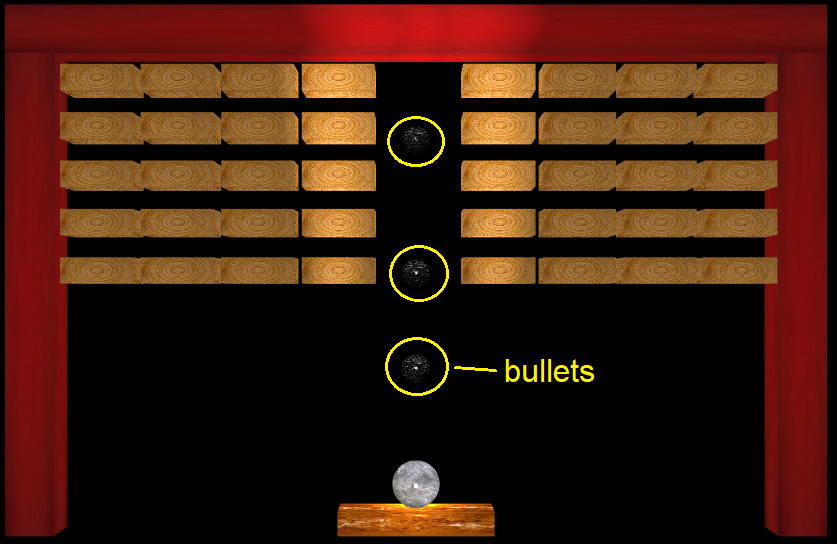
\includegraphics[width=0.7\textwidth]{Images/bullets.png}
	\caption{Image showing the bullets in the game}
\end{figure}